
\subsection*{Permutation Example}

%%%Insert this to get the typewriter font so it looks like a real movie script
{\ttfamily
\fontdimen2\font=0.4em
\fontdimen3\font=0.2em
\fontdimen4\font=0.1em
\fontdimen7\font=0.1em
\hyphenchar\font=`\-


\hypertarget{scripts_elementary_matrices_permutations}{Lets try to get the hang of }permutations. A permutation is a function which scrambles things. Suppose we had

\begin{center}
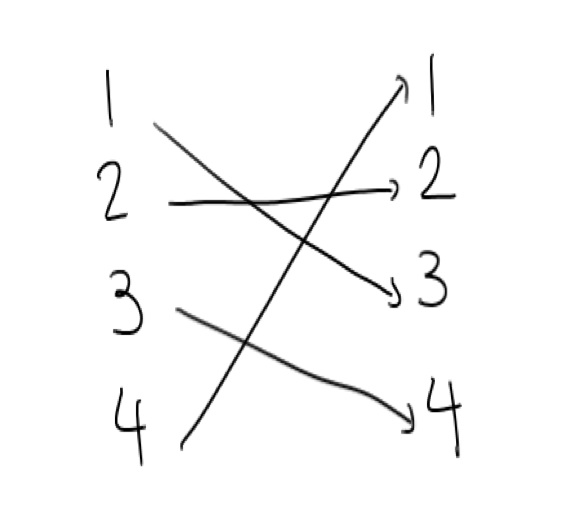
\includegraphics[scale=.35]{permutation_1.jpg}
\end{center}

 This looks like a function $\sigma$ that has values
 \[ \sigma(1) =3 ,\  \sigma(2) =2 ,\ \sigma(3) =4 ,\ \sigma(4) = 1\, .\]
 
 Then we could write this as
\[
\begin{bmatrix}
\mc1 & \mc2 & \mc3 & \mc4\\
\sigma(1) & \sigma(2) & \sigma(3) & \sigma(4)
\end{bmatrix}
= \begin{bmatrix}
1 & 2 & 3 & 4 \\
3 & 2 & 4 & 1 
\end{bmatrix}
\]
We could write this permutation in two steps by saying that first we swap 3 and 4, and then we swap 1 and 3. The order here is important.

\begin{center}
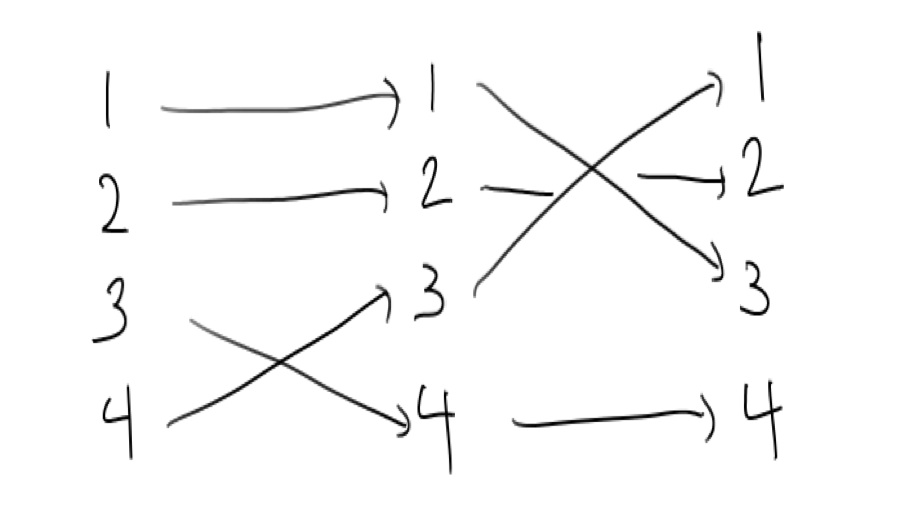
\includegraphics[scale=.35]{permutation_2.jpg}
\end{center}
This is an even permutation, since the number of swaps we used is two (an even number).
} % Closing bracket for font

%\newpage
